\documentclass{sig-alternate-10pt}
\usepackage{url}
\usepackage{framed}
\usepackage{amsmath}% http://ctan.org/pkg/amsmath
\usepackage[ruled]{algorithm2e}
\usepackage{graphicx}
\usepackage{comment}
\usepackage{hyperref}
\usepackage{authblk}
\usepackage{soul}
\usepackage{color}
\usepackage[font=footnotesize,labelfont=bf]{caption}
\usepackage[nameinlink]{cleveref}
\usepackage{xparse}% http://ctan.org/pkg/xparse
\NewDocumentCommand{\ceil}{s O{} m}{%
  \IfBooleanTF{#1} % starred
    {\left\lceil#3\right\rceil} % \ceil*[..]{..}
    {#2\lceil#3#2\rceil} % \ceil[..]{..}
}

\newcommand{\xin}[1]{\textcolor{red}{(XIN: #1)}}
\newcommand{\kelvin}[1]{\textcolor{blue}{(KELVIN: #1)}}
\newcommand{\Note}[1]{\textcolor{green}{(Note: #1)}}


\DeclareMathOperator*{\argmin}{arg\,min}

\begin{document}

\title{OpenCell: Exposing Cellular Performance Metrics for DASH-based Video}
\author[1]{\large X. Kelvin Zou\thanks{The work is done when Kelvin Zou is interning at AT\&T lab} }
\author[1]{\large Xin Jin}
\author[2]{\large Jeffery Erman}
\author[2]{\large Vijay Gopalakrishnan}
\author[2]{\large Emir Halepovic}
\author[2]{\large Rittwik Jana}
\author[1]{\large Jennifer Rexford}
\author[2]{\large Rakesh Sinha}
\affil[1]{ Department of Computer Science, Princeton University} \affil[2]{ AT\&T Lab, Bedminster}
\affil[1]{\texttt{\{xuanz, xinjin, jrex\}@cs.princeton.edu}} \affil[2]{\texttt{\{erman, gvijay, emir, rjana, sinha\}@research.att.com}}


\maketitle


%\begin{abstract}
%...
%\end{abstract}
\section{Introduction}
Video streaming has been the dominant factor in cellular networks, it consists
up to 40\% of the traffic peak load~\cite{LTENetwork, VideoMeasureatt}. Although
the video streaming has become one big part of cellular networks, the
performance for video streaming is not promising. Unique characteristics from
the cellular networks, such as bandwidth un-predictability over short period of
time due to handoff or fading effects, create a challenge for a satisfactory
video streaming service. 

Most of the current video streaming services are using DASH (\textbf{D}ynamic
\textbf{A}daptation \textbf{S}treaming over \textbf{H}TTP)\cite{DASH} based
end-to-end approaches. It uses chunk-based downloading and adjusts its video
streaming bit rate based on the play progress and the monitored bandwidth. The
application stitches video chunks together to provide a continuous playback.
However most of the video streaming service are not tailored for cellular networks, and they suffer from a conservative estimation and oscillation\cite{BBA,Festive, QDASH} .The reason for this is the lack of knowledge for the network condition. 
Some low layer connection information such as signal information is hard to access from application layer without root access.
Some mechanisms like Sprout\cite{Sprout} have been proposed to estimate link throughput, however it aims to reduce the packet delay while trading off the throughput, and need continuously saturate the link, which can be hardly used in video streaming case where downloading is periodical\cite{OnOff}.   
%For TCP throughput, the application need constantly saturate the link for a better estimation and the estimation takes a long time to converge, which can be hardly used in video streaming case where downloading is periodical\cite{OnOff,Sprout}. 
\xin{Not sure if this is correct. Can they be collected from end
hosts? Cite some papers or explain why it's hard}, \kelvin{ how is this sounds like now?}

On the other hand, a cellular network service provider has much better knowledge of the connection
conditions for the clients via monitoring, as the last mile has long been identified as the
bottleneck\cite{LASTMILE}. Cellular ISPs also know the number of
active users in each cell and the scheduling system, and thus can make more
precise predictions in terms of available bandwidth. In fact, many key statistics can be easily and some are
already being collected within carriers. 

Given cellular carrier's advantages, AVIS\cite{Avis} proposes an in-network video streaming framework where the network makes decision. 
Nevertheless it also suffers from some constraints. First it
lacks the application knowledge of play progress and may lead to re-buffering. 
Second different users may have different subscription
policies w.r.t. video streaming service and streaming service providers may
hesitate to share it with ISPs. Users may also have data budget concerns. Last
but not least, it may require the modification of the cellular scheduling system and that
may not be practical since most are using pre-installed
vendor-specific scheduler. 

To address the issue, we propose a novel cellular network design that exposes our in-network information to the video streaming service. By doing so video streaming service can play at higher quality and reduce the amount of chunk prefetching. There are three main contributions in this paper:
\begin{itemize}
\item Design a scalable architecture to compute KPIs(key performance indicators) and expose them to video streaming providers on the fly.
\item Conduct a measurement study to show the predictability of user channel quality and cell loads. 
\item Design an algorithm to show that by using the KPIs we have a significant improvement in video streaming service.
\end{itemize}

This paper introduces a scalable architecture to compute the bandwidth and expose the KPIs to the service provider in \autoref{sec:Architecture} and then we conduct a preliminary measurement study of predictability of available bandwidth in \autoref{sec:prediction}. We propose our new optimization algorithm in \autoref{sec:optimization} and show our results in \autoref{sec:evaluation}. This paper concludes in \autoref{sec:conclusion}. 



%\section{Related Work} \label{sec:relatedwork}
\emph{Video streaming:} in-network approaches like AVIS \cite{Avis} have its own video chunk download scheduler and it strikes a balance between fairness, efficiency and stability among users. However it overwrites the user request and fails to handle handoff situations. In addition, AVIS lacks the insight of client video buffer occupancy and only prefetches the next chunk, which may lead to excessive rebuffering. 

\emph{Network API/KPIs:} PANE \cite{PANE} extracts SDN APIs and exposes it to users to achieve a better efficiency, security or predictable behavior. Hadoop-OFN (openflow enabled) \cite{INFOBOX} uses SDN to query performance metrics and adjust the network scheduler to achieve higher Hadoop task performance. However both are domain specific approaches for datacenter or enterprise network.
 



\begin{comment}
\section{Background}
We explain  LTE network architecture and scheduling in \autoref{subsec:ltenet} and the video streaming service in \autoref{subsec:streaming}.
\subsection{LTE Network}\label{subsec:ltenet}

\emph{The architecture:} System Architecture Evolution (SAE) is the core network architecture of LTE wireless communication standard. SAE consists of two parts: Radio Access Network(RAN) and Evolved Packet Core(EPC). EPC has several parts including Mobility Management Entity(MME), Serving Gateway and PDN Gateway. 

\emph{The proportional fair scheduler:} the LTE networks are using Orthogonal Frequency-Division Multiuser Access(OFDMA) scheme to achieve high spectrum efficiency. To achieve multiuser diversity, eNodeBs are running variations of proportional fair scheduling system. A basic \textit{proportional fair scheduler} works as the following: eNodeBs obtain the feedback from each user about their instantaneous channel quality conditions (CQ) in terms of encoding rate per resource block, and take the ratio between it and historial mean of CQ and pick the user with the maximum ratio. In a static model over a long term, each user will get 1/N share of resource blocks if N is the static number of users in the cell, a dynamic model also has a similar result\cite{PFINFOCOM}. The maximum bandwidth for each user in a cell is a function of: $T$-number of resource blocks in the cell, $N$-number of users in the cell, and $\mathbf{CQ}$-channel quality vector for all users; so maximum bandwidth vector for all users $\mathbf{BW} = f(T, N, \mathbf{CQ})$. We do not directly address $f(T, N, \mathbf{CQ})$ function in this paper as it is vendor-specific and mostly it is close to the basic PF scheduler. In the rest of the paper we assume a simple PF scheduler, that is $\mathbf{BW} = f(T, N, \mathbf{CQ})=\frac{T}{N}*\mathbf{CQ}$. Among the three variables, $T$ is predetermined by the hardware, $N$ and $\mathbf{CQ}$ are the two factors we need to predict. 

\subsection{Video Streaming}\label{subsec:streaming}
Two unique features for state-of-the-art video streaming technique are (i) \emph{chunk-based download and play}, and (ii) \emph{dynamic play bit rate selection}. 

\emph{Chunk-based Download and Play:} most video streaming service providers including Netflix and YouTube are downloading and playing in chunks. A video is divided into hundreds to thousands of chunks, and each chunk is several seconds long. The download has an on-off behavior\cite{OnOff}: e.g., the client keeps moving the download point based on play progress, the download can be ahead of play progress with a relatively constant time window (usually at minute level), or dynamic window size(e.g., for YouTube it is $0.25 * PlayTime$) so the video play sessions can be resilient to some network congestion and temporary low throughput. It downloads the whole chunk when the chunk falls in the download sliding window, and cannot play the chunk until the chunk is fully downloaded. 

\emph{Dynamic Play Bit Rate Selection:} each video chunk is encoded in several bit rates, a higher bit rate means a better quality. Video streaming applications select a certain bit rate for each chunk to download, based on some utility function of both efficiency and stability. A video play session can consist of chunks with different bit rates and the video player will stitch the chunks together seamlessly. 

A video streaming application essentially needs to make two decisions: when and which play bit rate to download and play. 
\end{comment}

\section{Architecture} \label{sec:Architecture}
This section starts with the architecture of a scalable prediction system in
\autoref{subsec:prediction_system}, and then we discuss the feasibility and
advantages of inline method to expose KPIs in \autoref{subsec:exposingAPI}.
\subsection{Scalable Prediction System} \label{subsec:prediction_system} We
propose a two-tiered system to implement an KPI computing system. We have a
proxy sitting at dataplane; and local and central bandwidth estimator at control
plane. The local bandwidth estimator communicates with eNodeBs and it takes
channel quality, number of active users, cell load and users' queue size etc.
information as inputs and compute the available bandwidth for each user. A local
bandwidth estimator is logically distributed in the RAN and thus can be easily
scale-out. Meanwhile the central bandwidth estimator sits in the core network
and it summarizes local BW estimation and MME Mobility information to compute
the final bandwidth prediction for a user. In most cases one local estimation is
enough, however in cases like handoff we need choose among several local
estimations. Central estimators can be
scale-out with MMEs. Our architecture is generic and able to integrate into both
3G and 4G networks. 

Once the computation work is finished, the central estimator sends the
information to the proxy. 
 
\begin{figure}[tb]\label{fig:Architecture}
 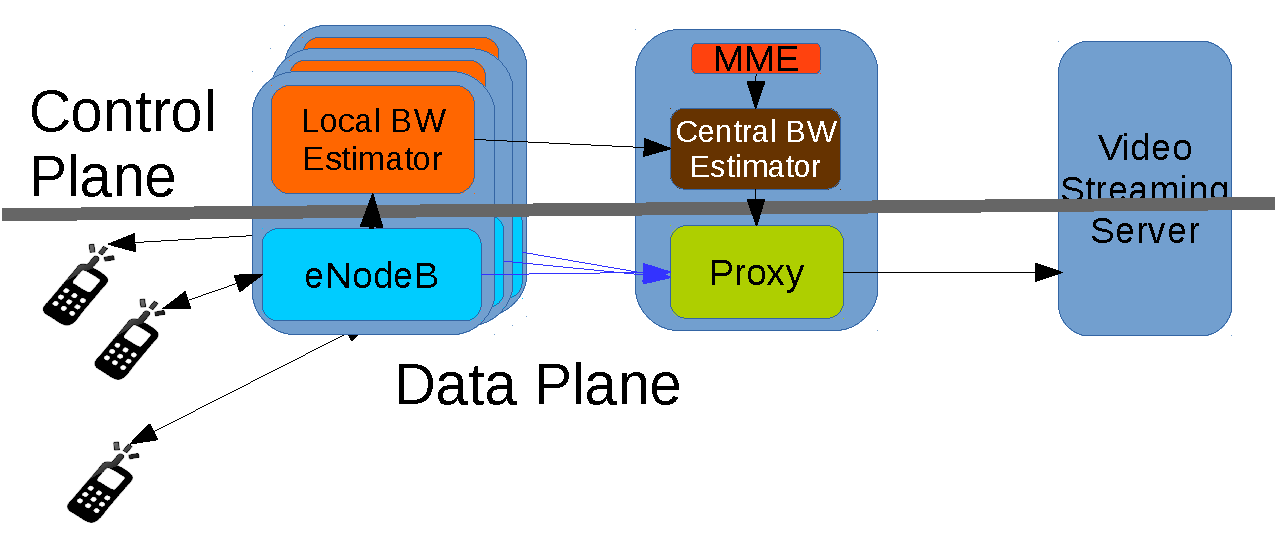
\includegraphics[width=\linewidth]{architecture2.pdf}
 \caption{Architecture for KPI Computing And Feedback}
\end{figure}


\subsection{KPI Exposure}\label{subsec:exposingAPI}
Current cellular networks already deploy proxies in the core network for
pacing purpose.\cite{UntoldMiddleBoxStory} It splits the TCP connection into two: server$\leftrightarrow
$proxy and proxy$\leftrightarrow $client. We can utilize the proxy for KPI
exposure. \emph{Sending to the server or the client?} We argue that exposing the
KPIs to the server causes less security concerns and network congestion. It also reduces the traffic in
the core network as sending to the client requires central estimator to send
back to local ones again. The downstream link carries majority of the traffic, upstream only has a small fraction of the traffic for feedback data. 
However since we let the server decide and the server in practice
may send back to the client's video play application. 

In terms of encoding the KPIs, there are several options: (i) in TCP; (ii) in
HTTP; and (iii) through a new connection. Inline methods have advantages over
new connection. First new connection method doubles the connections between the
server and the proxy. Second in practice CDNs are using public IPs, and the
video streaming connection and metric exposure connection may be directed to different private servers in CDN
load balancer. Inline methods both have some disadvantages. 
If we encode it into TCP option field, any middleboxes on the Internet may modify/drop the option field. 
The HTTP header may not be accessible since many streaming
services are using secure encypted HTTP. Modifying HTTP header also requires DPI, which has a higher overhead than changing TCP.
\begin{figure}[t]\label{fig:Datagram}
 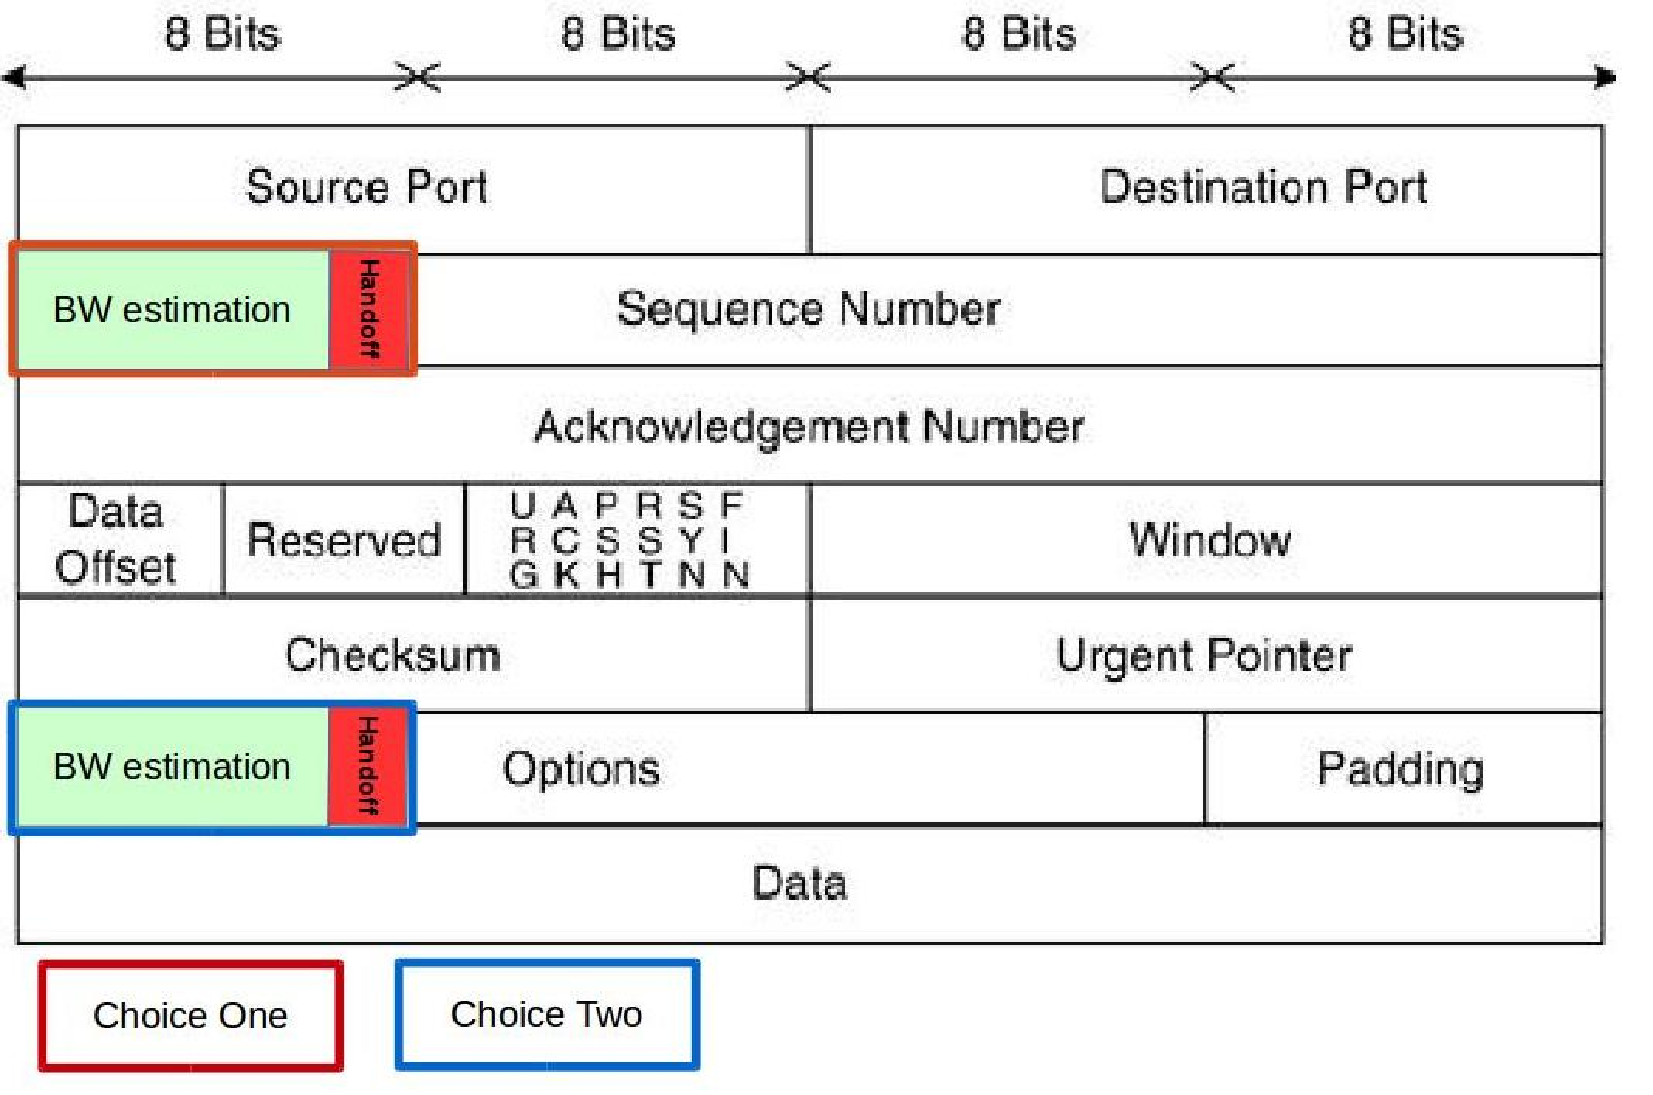
\includegraphics[width=\linewidth]{datagram.pdf}
 \caption{Datagram for exposing KPIs, it can be encoded in either option field or sequence number}
\end{figure}

One alternative approach is to encode in sequence number, if both content providers and cellular service providers are willing to collaborate. Since sequence number filed has 32 bits, we can reserve 8 bits for KPI exposure. In particular, we can use 7 bits for a floating number and 1 bit for handoff. Seven bits can be divided into integer and fractional parts, 3 bits for integer and 4 bits for fractional, it has a precision of 0.063 Mbps, or 63 Kbps and a maximum value of 8.94 Mbps, which is sufficient for today's video streaming bit rate selection where the range is bewteen 0.2 to 4 Mbps.
At the same time it can still support 16 million packets before wrapping around. The bandwidth estimation is close to random so it holds the random feature of initial sequence number.

\xin{Would any middleboxes on the
Internet (between the proxy and the server) modify/drop the TCP option fields?}

\xin{Can we say a bit more about API here? What do the APIs look like? Give an
example and show how it is encoded in TCP option field.}


\section{Measurement study and Key metrics prediction}\label{sec:prediction}
In \autoref{subsec:ltenet} we show in proportional fair scheduler the available bandwidth for each user is a function of (i) number of users in each cell, and (ii) the channel quality for each user, so the predictability of the two determines the estimated bandwidth. In this section we conduct an extensive measurement study to show the predictability of the link channel quality and the load on eNodeBs in \autoref{subsec:Prediction}. 

The traces are collected in Jun and July 2014 over several geolocations in the United States from one major 4G network carrier, it covers more than half million users and over 2000 eNodeBs. The traces have been anonymized before handing to us for privacy reasons. 

\subsection{Proportional Fair Scheduler}\label{subsec:ltenet}
3G ad 4G networks are using Orthogonal Frequency-Division Multiuser Access(OFDMA) scheme to achieve high spectrum efficiency. To achieve multiuser diversity, NodeBs and eNodeBs are running variations of proportional fair scheduling system. A basic \textit{proportional fair scheduler} works as the following: eNodeBs obtain the feedback from each user about their instantaneous channel quality conditions (CQ) in terms of encoding rate per resource block, and take the ratio between it and historical mean of CQ and pick the user with the maximum ratio. In a static model over a long term, each user will get 1/N share of resource blocks if N is the static number of users in the cell, a dynamic model also has a similar result\cite{PFINFOCOM}. The maximum bandwidth for each user in a cell is a function of: $T$-number of resource blocks in the cell, $N$-number of users in the cell, and $\mathbf{CQ}$-channel quality vector for all users; so maximum bandwidth vector for all users $\mathbf{BW} = f(T, N, \mathbf{CQ})$. We do not directly address $f(T, N, \mathbf{CQ})$ function in this paper as it is a vendor-specific PF-based scheduler. In the rest of the paper we assume a simple PF scheduler model, that is $\mathbf{BW} = f(T, N, \mathbf{CQ})=\frac{T}{N}*\mathbf{CQ}$. Among the three variables, $T$ is predetermined by the hardware, $N$ and $\mathbf{CQ}$ are the two factors we need to predict. 

\subsection{Bandwidth Estimation} \label{subsec:Prediction}


\subsubsection{Predictability}
First we define criteria for predictability: (1) Mean Absolute Percentage Error (MAPE); and (2) $\sum\text{MPE}_t$; where MPE stands for Mean Percentage Error. The reason for (1) is to minimize the side effect it gives to the video streaming application for each prediction it makes, and the reason for (2) is to avoid a biased prediction. For our domain specific application, (2) is especially important since (i) short term prediction error can be absorbed by the client playback buffer, and (ii) long term prediction should compensate the short term error, i.e., we can underestimate at time t and overestimate at time t+1 and the two errors are offset in application decision making. 


\subsubsection{Cell Load}\label{subsec:NUser}
We measured the number of active users in each cell from the same trace as mentioned above. The trace is collected from UE's RSRQ reports to eNodeBs. In a simple model if a user reports RSRQ in a one-second interval, we assume that user is active in that second. 

\begin{figure}[t]
\centering
 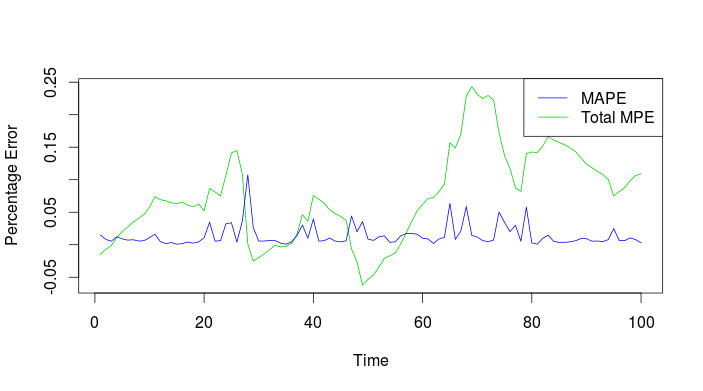
\includegraphics[width=0.8\linewidth]{pictures/MPE.png}
\caption{Error Analysis for Cell Load} \label{fig:NAIVEMPE}
\end{figure}

Although we predict the number of active users, we use the inverse value to compute the available bandwidth so MAPE=$ |\frac{1}{N_{true}} - \frac{1}{N_{pred}}| *N_{true}$, and $\text{MPE}_t=(\frac{1}{N^t_{true}} - \frac{1}{N^t_{pred}})*N^t_{true}$. ARIMA (auto-regressive integrated moving average) model can predict the number of active users with a fair accuracy, as it fits well with a stochastic model. We use auto.arima function in R ``forecast'' package to fit the best ARIMA model, and set the sliding time window to 15 seconds in both here and the following section. In fact for a moderate to heavy loaded cell a random walk, or ARIMA(0,1,0) occurs the most often. 

We plot MAPE and total MPE for one cell in a two minutes span in \autoref{fig:NAIVEMPE}, as we can see that the prediction has fairly small miscalculation at each step, and the total MPE $\sum$MPE$_t$ may oscillate to a greater positive or negative value. 
\begin{figure}[t]
\centering
 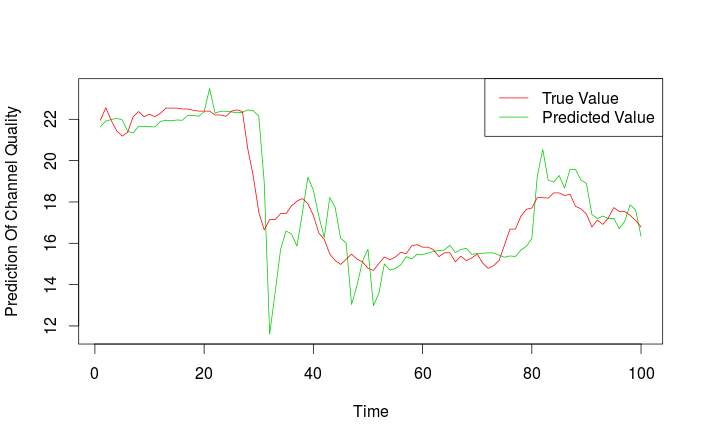
\includegraphics[width=0.8\linewidth]{pictures/prediction.png}
\caption{One sample prediction for channel quality: the algorithm makes a conservative estimation for channel quality once  it detects a great overestimation at 30s to minimize the total error} \label{fig:prediction}
\end{figure}
\subsubsection{Channel Quality}\label{subsec:CQ}
One unique characteristic for cellular network is the high mobility and this causes the link quality to fluctuate to a certain extent.

\emph{RSRQ:} Reference Signal Received Quality, is the key metric for the LTE wireless channel. RSRQ senses the load from other users in the same cell and the neighboring cells, and is indexed in 0-34 integer numbers; a higher number indicates a better link quality. RSRQ values can be mapped to certain encoding rate.
\begin{comment}
\emph{Data characteristic:} we find most of the users have fairly stable link quality, 54.6\% of the users have a CV (co-efficiency of variation) in terms of RSRQ within 0.2, but 3.6\% of the users have very dynamic link with a CV higher than 1. \emph{The Occurrence of Handoff}: in the dataset, handoff occurs for 30.7\% of the users, and average handoff occurrence is 2.2 times. Through further investigation, we found repetitive switch between two or three neighboring cells is quite often in our dataset, mostly due to similar RSRQs ($\Delta RSRQ<5$) from both cells. 
\end{comment}

Unlike Cell Load, the channel quality pattern is constantly switching between different ARIMA models when we apply auto.arima, and the prediction may keep over or under-estimating, in other words, the prediction may be biased. To address this problem, we add an auto-adjustment in prediction algorithm to keep the total error small. 

Through replay 50 random traces where the UEs are active for more than 100 seconds, we found that MAPE$<0.2$ for almost all the users, but $\sum\text{MPE}>0.5$ is in fact quite often. Without our auto-adjustment, $\sum\text{MPE}>1$ can also happen. 

The above results give us great insights in terms of prediction accuracy: a prediction can be 80\% accurate for each time segment while the cumulative error can be as much as 50\% of one time segment's bandwidth. 










\begin{comment}

\section{Design} \label{sec:optimization}
In this section, we explain the reason to choose an \textbf{\emph{end-to-end decision making with in-network knowledge}} model in section \ref{designchoice}, we then explain the our architecture in section \ref{architecture}. 
%introduce performance metrics in section \ref{metrics} and 

\subsection{Who decides the video streaming?}\label{designchoice}
For video streaming service decision making, there are three different models: \emph{In-network}, \emph{strictly end-to-end} and \emph{End-to-end with in-network knowledge}. 

\emph{In-network techniques} make decisions for users: it selects the video bit rate and schedule the download for users based on its knowledge of the network condition. However in-network approaches lack the insight of the video play progress, e.g., video buffer occupancy since it does not deal with any video decoding. Aside from technical reasons, here are several privacy/policy reasons for not doing this: most content providers are using encrypted http connections which ISPs cannot access; users may be concerned about their data budgets and thus not choose high bit rate; or content providers have different video play bit rate policies for different users based on their subscription contracts. 

\emph{End-to-end techniques} probe the network condition based on round trip time (RTT) and historical throughput, however existence of the proxy makes the RTT very inaccurate as it splits tcp connections. The dynamic nature of the wireless link makes historical data unable to capture the link behavior, e.g. the available bandwidth may plummet due to fading effects or handoff and recovers very soon after, current end-to-end approaches fail to react to those scenarios in most cases.

\emph{End-to-end with in-network knowledge} model addresses the above issues: instead of making the decision for the client; the network helps video streaming service make better decisions via offering some key performance metrics about the network condition, such as available throughput and handoff. 

Though an end-to-end with in-network knowledge approach has advantages over the other two, we still need to address the problem of how to expose the in-network knowledge in a least intrusive way in a scalable manner. 







\subsection{Architecture}\label{architecture}

We propose a two-tiered system for to implement OpenCell system. The two parts sit in RAN and EPC respectively. 

At the lower tier we have bandwidth estimator for each eNodeB. Estimating link channel quality and cell load is much more scalable if if we compute it at eNodeBs, since there are only hundreds of users at each cell, while aggregated number of users for a SGW can be tens of thousands. Making an estimation at second level means for each user the computational cycle is ~1 $ms$ if sitting at eNodeBs and ~10  $\mu s$ if sitting at Serving Gateway. Processing the raw information such as RSRQ from eNodeBs and extract it as estimated bandwidth also reduces the extra traffic generated for message passing. 

At the higher tier, the information inferred at eNodeBs are received at the proxy, and combined with handoff information, we make a final estimation of available bandwidth for each user and then expose this piece of information to application service providers by some means. The architecture is in figure \ref{cellular}.

\begin{figure}[t]\label{cellular}
\begin{minipage}[b]{\linewidth}
\centering
 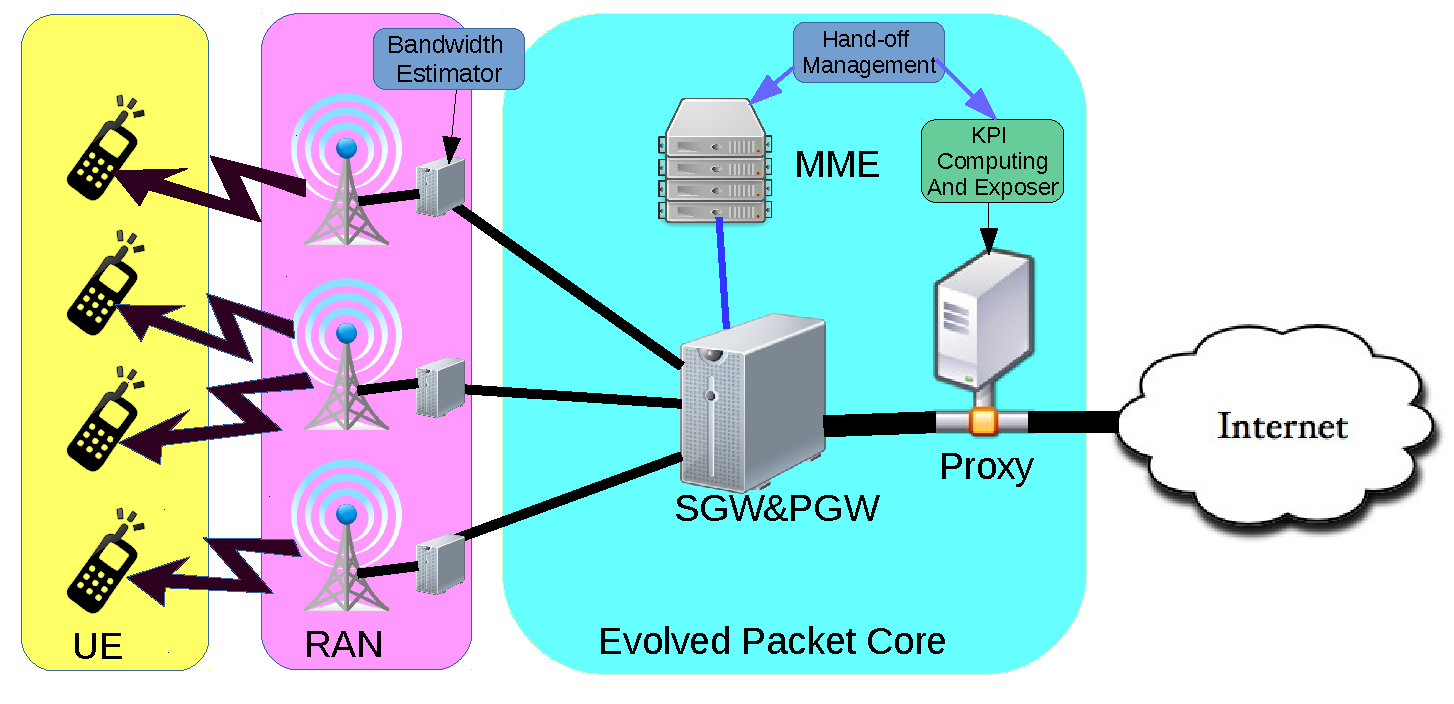
\includegraphics[width=\linewidth]{cellular.pdf}
\end{minipage}
\caption{OpenCell Design}
\end{figure}

In terms of how to expose the API information, there are three options: encapsulation (i) at TCP/IP layer, (ii) at application layer; and (iii) using a distinct channel. Each approach has its pros and cons, for example TCP/IP layer does not require DPI but the fields used for encapsulation might be overwritten deep in the network from middleboxes. Using distinct channel does not suffer either problem but it requires application service providers' cooperation. We are still weighing between the options and leave this as a future problem. 



\end{comment}

\section{Video optimization algorithms}\label{sec:optimization}
In this section we first define performance metrics in \autoref{subsec:metrics}. We give an offline optimization to define the video quality (efficiency) upper bound where we are aware of the available bandwidth for the whole session in \autoref{subsec:offline}.  Given the exposed APIs, we then design a new video streaming algorithm in section \ref{subsec:online},  to demonstrate the benefits of newly OpenCell.
\begin{table*}
\begin{tabular} {|c |c |}
\hline
Notation&Meaning\\ \hline
$T$ &the number of time segments\\ \hline
$M$ &the number of video quality levels (encoding bit rates)\\ \hline
$R_i$& the rate for the video with $i^{th}$ highest encoding bit rate\\ \hline
$x_i^t$&indicator of encoding of $R_i$ video play rate at time t, used in offline algorithm \\ \hline
$E$& utilization of used bandwidth over maximum available bandwidth \\ \hline
$\phi^t$ &the number of quality jumps between two consecutive chunks at time t\\ \hline
$C $ &the estimated capacity\\ \hline
$B $ &the buffer occupancy(seconds of video) \\ \hline
$z $ &the maximum buffer size (seconds of video) \\ \hline
$B_{rec} $ &the recommended buffer size (seconds of video) \\ \hline
\end{tabular}
\centering
\caption{Variables for Optimization}
\end{table*}


\subsection{Performance Metrics}\label{subsec:metrics}
To help us understand what extra benefit we can achieve from new information in the cooperative model, we define \emph{three} metrics for the performance of video streaming given a known network. These metrics have been extensively studies in various approaches and here we use them as a benchmark to test our new model\cite{Qava, Avis,VideoMeasurement, Festive}.

\begin{enumerate}
\item\textit{Quality}: as the video download is chunk-based, a video session can consist of chunks with different qualities (bit rates). The video player should download the chunk with the highest possible quality based on available bandwidth at each download point to give user better quality experience. 

\item\textit{Stability}: From viewer's perspective, constant switches between different qualities are distracting and not desirable. To assess the stability of video streaming, we use the concept of fluctuation: it is the the number of jumps difference between two consecutive sessions, \emph{fluctuation cost} at time t: $\phi^t =  \|i*x_i^t - i*x_i^{t-1}\|$.

\item\textit{Interruption}: Video play should not be halted for fetching video chunks, otherwise user experience will be severely degraded. Video play interruptions affect the user engagement and results in early abandonment of the video play. Video streaming players usually buffer extra chunks to absorb any sudden drop on the link capacity. We use the frequency of interruptions over play time as an indication for interruption; $\beta = \frac{N_{interrupt}}{PlayTime}$.
\end{enumerate}

\subsection{Metrics Upper Bound}\label{subsec:offline}
Upper bounds for metrics like stability and interruption are straightforward, they should be zero in an intuitive sense. We will formulate a way to find video quality (play efficiency) upper bound, e.g., given the available bandwidth the whole video play session 1 to T, we ask for the optimal video download and play to best utilize the available bandwidth. We prioritize zero-interruption and we ignore the stability factor. 

To capture zero-interruption, at each time segment the download should always at least be equal to video played (assume at the initial state the client video buffer contains one chunk ahead of playing), i.e., $\sum \limits_{t=1}^\tau R_i * x_i^t\leq\sum\limits_{t=1}^\tau C^t$ for $\forall \tau \in \{1, \dots, T\}$. In terms of measuring the quality (play efficiency) at the end of a video session, the play efficiency equals to the total utilization of the available bandwidth over time period $[1:T]$, we use ratio of the throughput used for video downloading and playing over the available bandwidth: $\bar{E}=(\sum\limits_{t=1}^T D^t)/(\sum\limits_{t=1}^T C^t)$.

\begin{subequations}
\begin{align*}
&\textsc{maximize }&\bar{E}\\ 
&\textsc{Subject to}\\
&\sum \limits_{t=1}^\tau  \sum \limits_{i=1}^M R_i \cdot x_i^t\leq\sum\limits_{t=1}^\tau C^t& \forall \tau \in \{1, \dots, T\}\\
&\sum \limits_{i=1}^M x_i^t =1\; and\;\; x_i^t = \{0,1\}&\forall t, \forall i
\end{align*}
\end{subequations}

\subsection{Continuous Online Algorithm} \label{subsec:online}
\begin{algorithm}[ht]
\SetAlgoLined
 \KwData{ $C$: Predicted available bandwidth\newline$B'$: Current buffer occupancy\newline$\Delta B$: Buffer occupancy change\newline$R_{cur}$: Current video bit rate}
 \KwResult{$Rate$: Rate for next chunk }
$Score = +\infty$\;
$ R_{rec}=\argmin (\frac{1}{E} + \beta*COST )$\;
 \uIf{$B'\leq B_{rec} $}{
\uIf{$R_{rec}<R_{cur} \&\& \Delta B<0$}{
$Rate = R_{rec}$
} 
\uIf{$R_{rec}>R_{cur}$}{
$Rate = R_{rec}$
}
\Else{
$Rate = R_{cur}$
}

 }
\Else{ 
\uIf{$B'\geq z$}{
Idle for $(B'-z)$ seconds\;
}
\uIf{$R_{rec}<R_{cur} \&\& \Delta B<-\frac{B_{rec}}{2}$}{
$Rate = R_{rec}$
} 
\uIf{$R_{rec}>R_{cur}$}{
$Rate = R_{rec}$
}
\Else{
$Rate = R_{cur}$
}
}

\caption{Rate Selection} \label{cap:algorithm}
\end{algorithm} 

In the online algorithm, we restrict ourselves to (i) at most prefetch $z$ seconds video chunks, and (ii) only gives available bandwidth forecast for one chunk time interval. Our algorithm is a joint optimization solution based on both the video buffer occupancy and the estimated bandwidth. 

State-of-the-art video streaming algorithms \cite{BBA, Festive} share great similarities in a few aspects: (i) deferred updates of video bit rate over link condition, (ii) periodic download if video buffer is full. Our design also applies the same concepts. We now focus on the three key metrics.

% \textbf{We also show that by integrating our KPIs existing algorithm can also improve its video streaming performance, but the improvement is limited by its mismatched design where KPIs were not considered. NOT DONE YET} 

For interruption, unlike quality and stability which can be easily quantized in the algorithm, we need take an alternative view via looking at the video buffer occupancy, in particular we should avoid the video buffer empty. There is a tradeoff between prefetching, quality and interruption. Prefetching many video chunks is (i) not efficient, as it conservatively downloads more video chunks and play at lower quality; and (ii) wasteful if the viewer abandons the vide session. We factor in the video buffer occupancy to adjust requested download bit rate. If the buffer occupancy is high we can take a risk to download at higher rate beyond the estimated bandwidth and if the buffer occupancy is low we may conservatively download at lower rate than estimation. The video buffer occupancy can be used as a discount/inflation factor for the estimated bandwidth: when the buffer occupancy is low, we use the discounted bandwidth estimation and download more chunks with lower rates to fill the buffer, when the buffer occupancy is high we use the inflated bandwidth to drain the buffer a little faster. We define inflation as a concave function: $f(B)= \log(1+\frac{B}{B_{rec}})$, where $B_{rec}$ is the recommended equilibrium buffer size.  

For stability, we use exponential penalty for play bit rate jump and define the fluctuation $COST = 2^{\phi} *e^{-\alpha *\Delta t}$. The reason is to discourage but not to disallow a jump of more than one level. We also add an exponential time decaying where $\Delta t$ represents the time interval since last bit rate changes and $\alpha$ is a tunable parameter to reflect the time significance. For efficiency, we take the inverse of link utilization over inflated bandwidth to penalize the under-utilized bandwidth: $\frac{1}{E} = \frac{C}{BitRate}*\log(1+\frac{B}{B_{rec}}) $. Combine this and the fluctuation cost with a tunable knot, we have a score function $Score= \frac{1}{E} + \beta*COST$. 


We use the bit rate= $\argmin{(Score)}$ as the recommended video bit rate. We further delay the video bit rate step up or step down based on $B$ buffer occupancy and $\Delta B$ buffer change from last chunk download via the following mechanism to absorb the high link fluctuation, while $Score$ function absorbs low and median bandwidth fluctuation. We divide the buffer occupancy into two zones: risky $[0,B_{rec}]$ and safe $[B_{rec},z]$. In risky zone, if the client video buffer is depleting, if $\Delta B>0$ we defer the video bit rate stepping down, as it may just be a short period of low throughput. When $B$ is in safe zone we take more risk and step down if $\Delta B <-\frac{B_{rec}}{2}$ which means if the buffer is depleting substantially and a preemptive action is needed before stepping into risk zone. Stepping up is allowed since in risky phase the bandwidth is already a discounted bandwidth, and in safe phase we have sufficient buffer. 
  
The online algorithm continuously estimates the bandwidth for the next time segment and then computes the cost score for each video bit rate, it selects the bit rate based on $Score$ and $\Delta B$, as shown in \autoref{cap:algorithm}.


%%%%%%%%%%%%%%%%%%%%%%%%%%%%%%%%%%%%%%%%%%%%%%%%%%%%%%%%%%%%%%
%Comment out, leave in case for future use!

\begin{comment}

\begin{algorithm}[h]
\SetAlgoLined
 \KwData{ $C$: Prediction available bandwidth\newline$C'$: Prediction lower bound with 90\% confidence\newline$B'$: Current buffer occupancy\newline$t_s$: Last time video has switched bit rate\newline$i'$: Current video bit rate}
 \KwResult{$Rate$: Rate for next chunk}
\uIf{$\frac{R_1}{C} \leq 1$}{
$Rate = R_1$\;} 
\Else{
$Score =0$\;
\For{i \leftarrow 1 to M} {
$\mathbb{E}[\Delta B] = \ceil{ (\frac{R_i}{C'}-1)\cdot 4} $\;
$\phi =|i-i'|$\;
$Score_i = \frac{R_i}{C} -\mathbb{E}[\Delta B] \cdot \frac{1}{B'} - \phi \cdot EXP(t_s-t_{now})$\;
\uIf{$Score\leq Score_i$}
{
$Score=Score_i$\;
$Rate = R_i$} 
}
}
\caption{Rate Selection}
\end{algorithm}


for (i) is that the cost of making bit rate jump should depend on when is the last time we make bit rate change. Tht cost for bit rate change should be less if the last bit rate change is long time ago. The reason for (ii) 
\begin{algorithm}[h]
\SetAlgoLined
 \KwData{ $C$: Link capacity for next 4 seconds\newline $B_{now}$: Current Buffer Occupancy\newline$V$: Reservior Size\newline $\Delta B$: buffer occupancy change in last time segment}
 \KwResult{$Rate$: Rate for next chunk }
% \BlankLine
\uIf{$B_{now}>V$}{
$Rate$ = BBA\_steady()} 
\Else{
$Rate_{infer} = \min\{Rate_{max}, 0.8*C \}$\;
\emph{if the buffer is filled at a certain pace, pick the inferred rate}\;
\uIf{$\Delta B >0.3(1-\frac{B_{now}}{V})*V$}{
$Rate = Rate_{infer}$
} \Else {\emph{Othewise, pick one level below}
$Rate = \max\{Rate_{min}, Rate_{infer-1}\}$
}
}
Update(Cushion Size, Reservior Size)\;
\caption{BBA(2) PLUS Rate Selection}
\end{algorithm}

\begin{algorithm}[h]
\SetAlgoLined
 \KwData{ $C$: Link capacity for next 4 seconds\newline $b_{ref}$: Computed bit rate\newline$b_{cur}$: Current play bit rate\newline$BitChangeTime$: last time bit rate change }
 \KwResult{$Rate$: Rate foralso next chunk}
 //Pick the bit rate right below link capacity, 0.9 is a factor for encoding overhead.
$b_{ref}= 0.9*\lfloor C \rfloor$\;

\uIf{$TimeNowlookahead-BitChangeTime>20$}{
\uIf{$b_{ref}\not = b_{cur}$}
{
$BitChangeTime = TimeNow$
}
\Return{$b_{ref}$}
} \Else{
$ score_{ref} = score_{e}(b_{ref}) +\alpha*score_{s}(b_{ref})$\;
$score_{cur} = score_{e}(b_{cur}) +\alpha*score_{s}(b_{cur})$
\uIf{$score_{ref} > score_{cur}$}{
$BitChangeTime = TimeNow$\;
\Return{$b_{ref}$}
} \Else {\Return{$b_{cur}$}}
}
\caption{FESTIVE PLUS Rate Selection}
\end{algorithm}


\subsubsection{FESTIVE+}
FESTIVE(Fairness, Efficient and Stable adapTIVE algorithm) algorithm\cite{Festive} assumes the following: there is a single bottleneck link in the network, which would be the wireless link in the cellular network, and the video downloading is very periodic, i.e., it has a noticeable on-off phase in terms of video chunk downloading. It has three components: 
\begin{enumerate}
 \item Select when the next chunk will be downloaded: it uses randomization of download start time ($t_{i}^{start}$) to avoid potential synchronization of congestion in the bottleneck link and increases the bandwidth estimation confidence. 
 \[
   t_{i+1}^{start}= 
\begin{cases}
    t_{i}^{end}, \; \;&\text{if}\;\; buffer_i < randbuf_i; \\
    t_{i}^{end}+ &buffer_i-randbuf_i,\;\; \text{  otherwise}
\end{cases}
\]

 \item Select a suitable bitrate for the next chunk: it uses delayed updates-if there has no play bit rate change in the last 20s, the streaming is free to change bit rates based on its bandwidth estimation. If an bit rate change is needed within 20 seconds, it has an efficiency cost $score_{e}{(b)}=|\frac{b}{\min{(w, b_{ref})}} -1|$, and a stability cost $score_{s}(b)=\begin{cases}
   2^n+1, \; \;&\text{if}\;\; b=b_{ref}; \\
     2^n, \; \;&\text{if}\;\; b=b_{cur};\\
\end{cases}$, and the combined score is linked by a tunable parameter $\alpha$, $b=argmin (score_{e}(b) +\alpha*score_{s}(b))$.
 
 \item Estimate the network bandwidth: it takes harmonic mean over the last 20s as an estimation for future bandwidth, since it is a more stable and conservative estimation.
 
\end{enumerate}
\emph{Our changes:} we make only one small change in their algorithm; (i) we replace harmonic mean with our KPI, which could be intepreted as a ground truth or very close estimation;(ii) we turn off the randomization since FESTIVE uses it to avoid inaccurate estimation while our model does not suffer this problem. We name our algorithm FESTIVE PLUS.

\end{comment}


 

\section{Evaluation} \label{sec:evaluation}
We conducted extensive simulations to verify our idea. The setup and baseline algorithms is in \autoref{sub:setup}. We show the improvement space in \autoref{sub:oracle} where the estimated bandwidth is from an oracle prediction and show our algorithm performs close-to-optimal in a noisy prediction scenario in \autoref{sub:noisy}. 

\subsection{Setup} \label{sub:setup}
 The available bandwidth traces are taken from one major U.S. 4G network carrier and MIT Sprout Project\cite{Sprout} and we cut each trace into 5-10 minutes long segments, as 80-90\% video sessions are shorter than 10 mins.\cite{ATTVIDEO} In total there are four 3G and 12 4G segments. We take 10 different video encoding rates from Netflix: $\{0.235,\dots, 4.3\}$ Mbps and we assume no variation in bit rates. 

We choose FESTIVE \cite{Festive} and BBA \cite{BBA} algorithms as baselines for comparison. FESTIVE solves the problem where there is one bottleneck link in the network shared via several video streaming users. It takes the harmonic mean of bandwidth over the last 20 video chunk downloads as reference and adds randomization into video chunk download scheduling to avoid a synchronized congestion. BBA class algorithms rely on video buffer occupancy as an implicit feedback of the network condition for video bit rate selection, and use a linear relation to the buffer occupancy to compute the desired rate. It also has a fast startup phase where it ramps up to a desirable play bit rate based on buffer occupancy growth rate. Throughout our experiments, we set the tunable knot for stability $\alpha =12 $ and bandwidth factor $p=1$, and in BBA we are using BBA(2) with $BufferReservior=90s$, $BufferCushion=136s$ and max buffer $z=240s$. In our approach we set recommended buffer size $t=60s$ and max buffer $z=240s$. Each video chunk is 4 seconds, which is a prevalent length for one major video streaming vendor. 



%\subsection{Algorithm Performance}



\begin{figure}[t]
 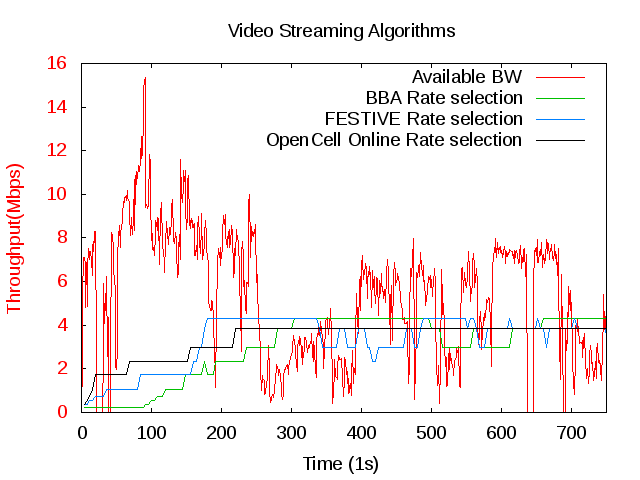
\includegraphics[width=\linewidth]{ATT.png}
 \caption{A sample trace from one major 4G network}
\end{figure}

\begin{table}[t]

\begin{tabular} {|c |c |c |c |}
\hline
 Improvement &Quality &Stability & Interruption\\ \hline
BBA(3G)  & 1.09x& 2.78x& 1x \\ \hline
FESTIVE(3G)    & 1.34x & 1.26x&5.5x\\ \hline
BBA(4G) & 1.16x& 2.1x& N/A \\ \hline
FESTIVE(4G) & 1.13x& 3.6x& N/A \\ \hline
\end{tabular}
\centering
\caption{Improvement with oracle estimator} \label{cap:table}
\end{table}


\subsection{Oracle Estimator}\label{sub:oracle}
In this section, the algorithm is using an "oracle" estimator, to show the space of improvement.

\emph{Key metrics improvement:} we measure three different metrics: quality (play efficiency), stability and interrupts. Play efficiency measures during the play session, the video downloaded and played vs available bandwidth. Stability measures the number of bit rate switches and interrupts measures the occurrence of interruption. Our algorithm outperforms the other two algorithms in all traces in terms of all three metrics, and the summary is in \autoref{cap:table}.

%\emph{Key metrics improvement:} we measure four different metrics: quality (play efficiency), stability and interrupts. Link utilization measures the total download vs available bandwidth, and the value is one if the link is constantly saturated. Play efficiency measures during the play session, the video downloaded and played vs available bandwidth, in the case without prefetched chunks, download utilization and play efficiency are equal. Stability measures the number of bit rate switches and interrupts measures the occurrence of interruption. Our algorithm outperforms the other two algorithms in all traces in terms of all four metrics, and the summary is in \autoref{cap:table}.

\emph{Prefetched buffer size}: we also compare the prefetched buffer size between BBA and our approach. FESTIVE is not client video buffer based solution and only adds randomized scheduling if it reaches a certain buffer level, we extend that buffer level to $z=240s$ download and see no difference in terms of its efficiency, stability or interruption, but we observe a little higher link utilization. Comparing BBA, we have reduced buffer size significantly by 20-30 seconds if we set $z=240$. We also notice no difference if we set $z=150$ in our new algorithm, however BBA suffers a higher oscillation in 4G traces. 


\emph{Comparison with Theoretical Max}: for a formulation in \autoref{subsec:offline}, we use IBM CPLEX to solve the mixed integer problem. We again replayed the 16 traces and the result shows that our approach can achieve 78.5\% close to the efficiency upperbound. In our offline algorithm one 3G trace has no feasible solution, and the reason is from the zero-interruption constraint, which also justifies the inevitability of interruption occurred in online algorithms. 

%\emph{Comparison with Modified FESTIVE}\Note{Not done yet!}: to show the performance gain is from both the novel algorithm and exposed extra KPIs, we also modified FESTIVE: we feed FESTIVE with a future bandwidth instead of using its harmonic mean estimation. 


\begin{table}[t]

\begin{tabular} {|c |c |c |c |}
\hline
 Improvement &Quality &Stability & Interruption\\ \hline
BBA(3G)  & 1.16x&1.6x &\textcolor{red}{0.9x} \\ \hline
FESTIVE(3G)& 1.40x &\textcolor{red}{0.86x}& 5x\\ \hline
BBA(4G) & 1.17x& 1.9x& N/A \\ \hline
FESTIVE(4G) & 1.14x& 3.4x& N/A \\ \hline
\end{tabular}
\centering
\caption{Improvement with noisy estimator} \label{cap:table2}
\end{table}

\subsection{Noisy Estimator}\label{sub:noisy}
We use a synthetic estimator for prediction and show that when the prediction is roughly accurate with a certain degree of error rate, our algorithm is robust to achieve a close-to-optimal performance. The key criterion for a good estimator is to have low error rate at each step and low to medium cumulative error rate over history. 

\emph{Noisy estimator}: we use a synthetic estimator to conduct a sensitive study for the new algorithm. The synthetic estimator makes prediction with a random factor in a N(1,0.2) distribution, means our prediction is $\geq$80\% accurate with 68\% chance, and $\geq 60\%$ accurate with 95\% chance. We run each syntheic estimator for 10 times for each trace and take the average. 

From \autoref{cap:table2} we can see that the quality is equal or even better, better quality is due to its higher sensitivity to high bandwidth estimations. However we lose some stability due to its unnecessary adjustments from inaccurate estimations, which leads to more frequent client play buffer changes. 


\section{Conclusion}\label{sec:conclusion}

 
 
\bibliographystyle{acm}
{\small
\bibliography{references}} 

\end{document}
